%_____________________________________________________________________________________________ 
% A Holistic Approach to Autonomic Self-Healing Cloud Computing Architecture
% Chapter 2 - 
% Fri Apr 19 12:50:42 IST 2013
%_____________________________________________________________________________________________
\chapter{Autonomic Self-Healing Architecture}
\section{Architecture Overview}
An autonomic mechanism will be used to deploy a monitoring system which will be responsible for collecting the resource utilization statistics of the remote hosts in the cloud. The collection of this data will be carried out periodically at regular intervals specified by the Autonomic Healing Engine. Each host will have a client version of the same monitoring system running as a daemon process. The client version of the monitoring system will send system resource utilization data to the monitoring system server application running on the Autonomic Healing Engine. The Autonomic Healing Engine  passes this data to a Fault Detection Engine. The Fault Detection Engine is responsible for analyzing the data received and deducing the correct action to be taken in order to avoid the fault. The Fault Detection Engine stores statistical data such as load on the CPU, traffic on the Network Interface Cards of the various hosts, RAM usage, frequency of disk operations, etc. The Autonomic Healing Engine detects the Process Imprint of the executing process. An action deciding mechanism is implemented within the Fault Detection Engine which makes use of the Process Imprints and Process Association Graphs of the processes which are running on various instances of the hosts in the cloud.
	\begin{figure}[t]
		\begin{center}
			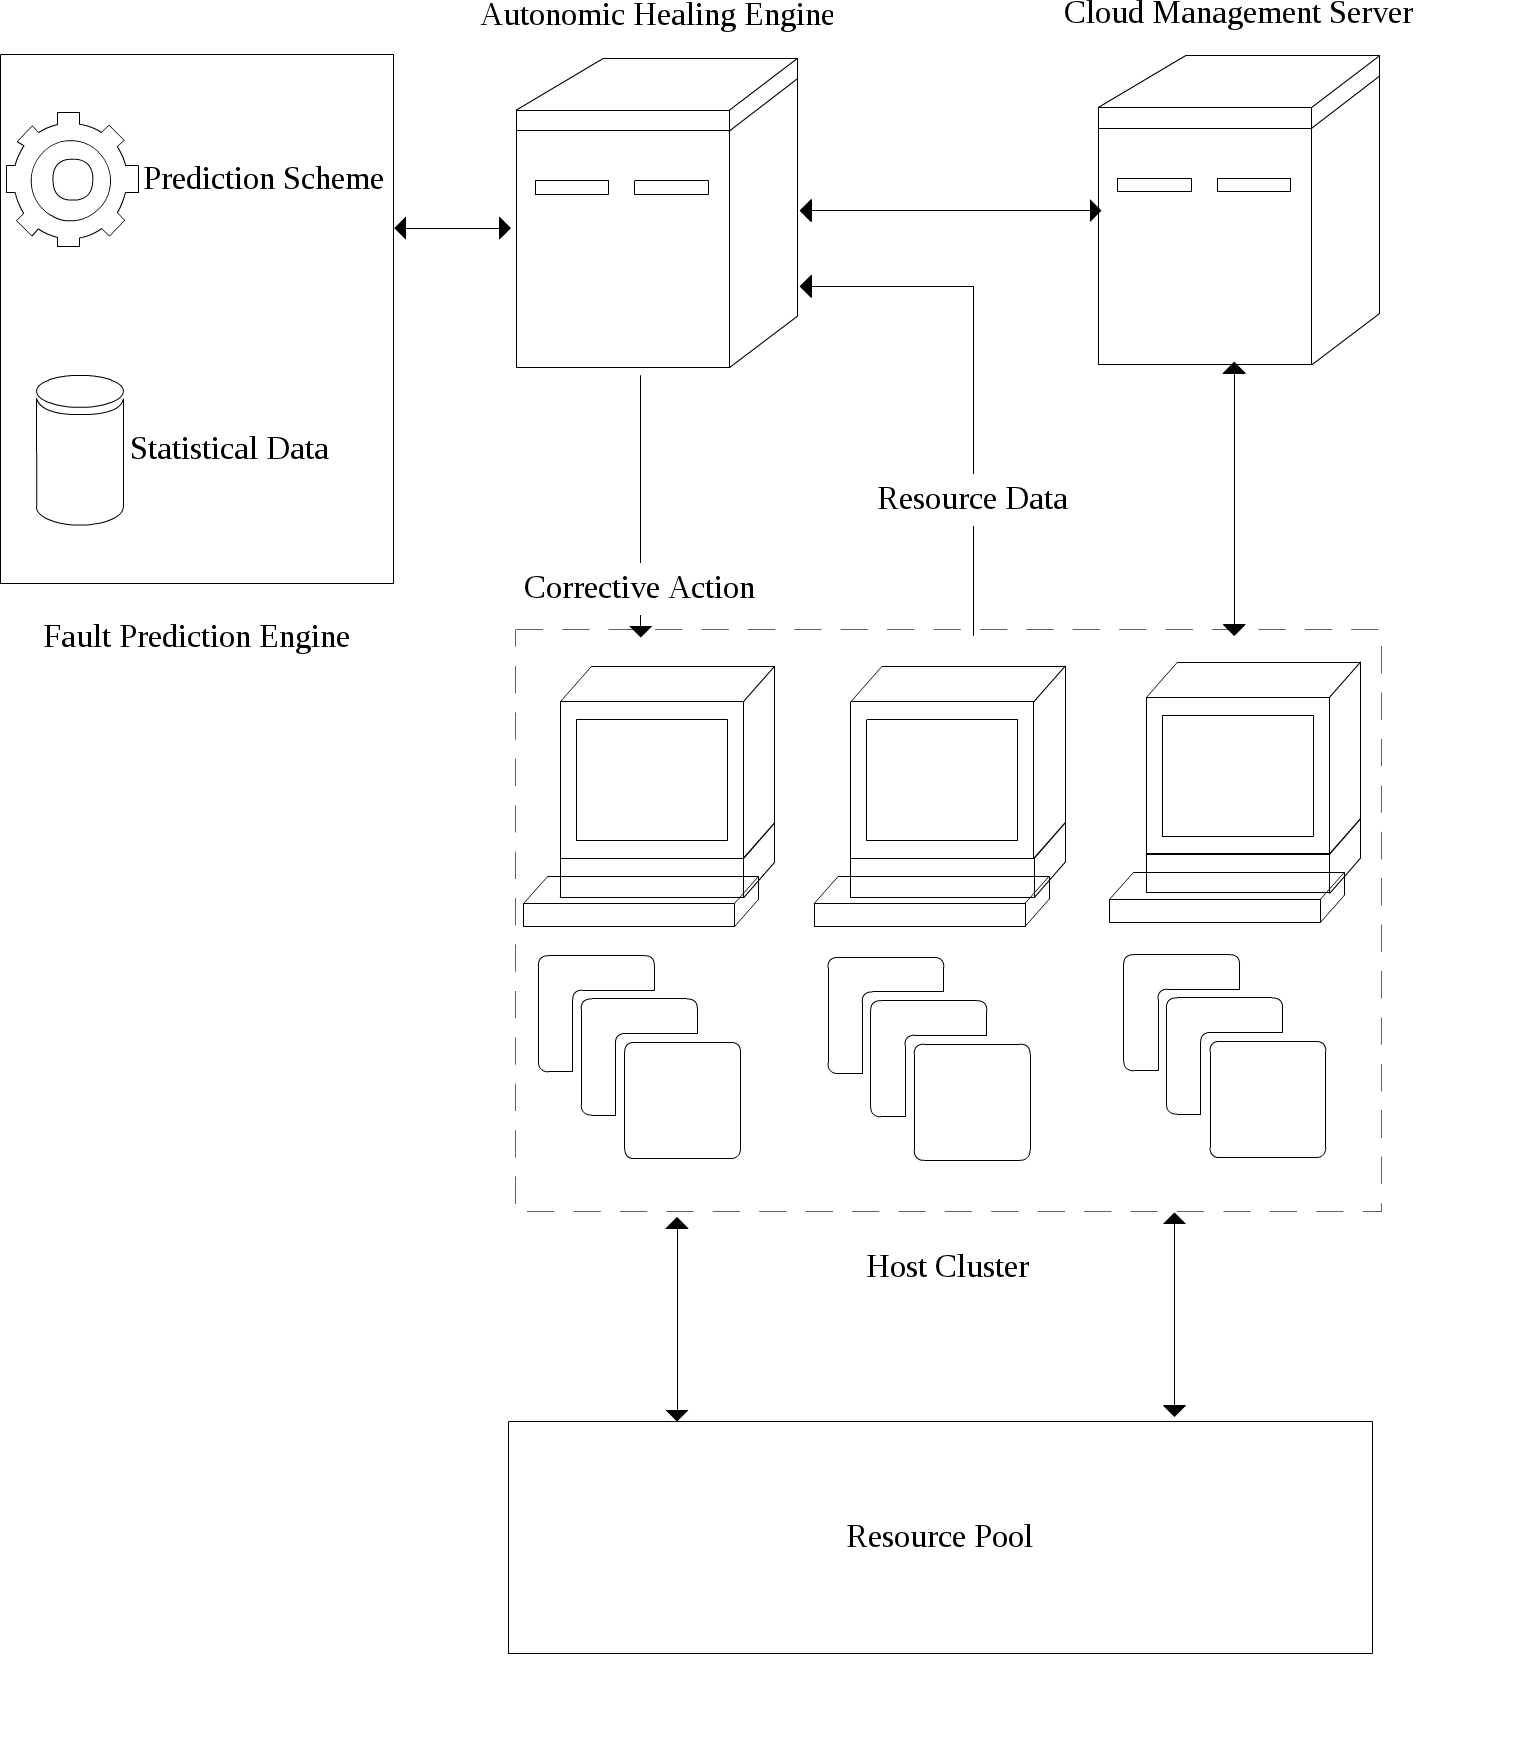
\includegraphics[width=10cm,height=10cm]{figures/cloud_architecture.eps} 
			\caption{\small \sl Autonomic Self-Healing Cloud Computing Architecture.\label{fig:Label6}} 
		\end{center} 
	\end{figure}
\section{Components}
\subsection{Resource Pool}
The Resource Pool consists of all the different resources that are allocated to the various virual machines that are executing on the cloud host cluster. These resources include computational power, network bandwidth, memory, storage capacity, etc.The host cluster uses this resource pool to provide for the virtual machines that are running on them.
\subsection{Host Cluster}
This consist of all the compute units. This provides for all the computing power in the cloud. The hosts though independent, are managed by the cloud management server. The host powers all the Virtual Machines(VMs from here on) through their respective hypervisor. These VMs are directly accessible to users.

The hosts have a monitoring agent installed on them. This monitoring agent monitors the system and the log messages and forwards these log messages to the autonomic healing engine.
\subsection{Cloud Management Server}
The cloud management server powers the cloud. It is the backbone and acts as a link between hosts and resources. Cloud management server provides a unified view of the entire computing environment and also provides various management consoles for easy management.
\subsection{Autonomic Healing Engine}
The autonomic healing engine acts as a middleware between the hosts cluster and the fault prediction engine. It receives the system log messages from the hosts cluster and forwards them to the fault prediction engine for analysis and storage. The autonomic healing engine also receives the analyzed information from the fault prediction engine. This information then helps the autonomic healing engine to decide the action to be taken in case of a possible fault.

The separation from the fault prediction engine allows for plugability. In essence, this means that the healing actions can be independent of the fault prediction scheme. The flexibility thus induced, helps to develop healing engines for an array of systems and thus makes the architecture truly holistic.
\subsection{Fault Prediction Engine}
The fault prediction engine analyses statistical data received from the autonomic healing engine. It uses data mining and machine learning techniques to recoqnize fault patterns and irregular behaviour in logs. It comprises of two parts
\subsubsection{Statistical Data}
This is the central data store that stores all previously analyzed results. This acts as the learning and trainset for the prediction scheme. Storing of previous data helps in analyzing change of events and also patterns in change of types of failures overtime.
\subsubsection{Prediction Scheme}
The failure prediction scheme incorporates various data mining techniques to predict failures by generating rules. This module is independent of the autonomic healing engine and thus can be upgraded with new and better algorithms transparently.
\section{Prediction Scheme}
We now present a high level diagram of the proposed fault prediction scheme. The scheme involves two parts: data scrubbing and the other for fault prediction. We used the RAS logs from the Blue Gene/L System available at ANL.\cite{FAILURE_1}\cite{BLUEGENE_1}\cite{BLUEGENE_2}\cite{FAILURE_4} More information about the data can be found in the Appendix.
\begin{figure}[t]
		\begin{center}
			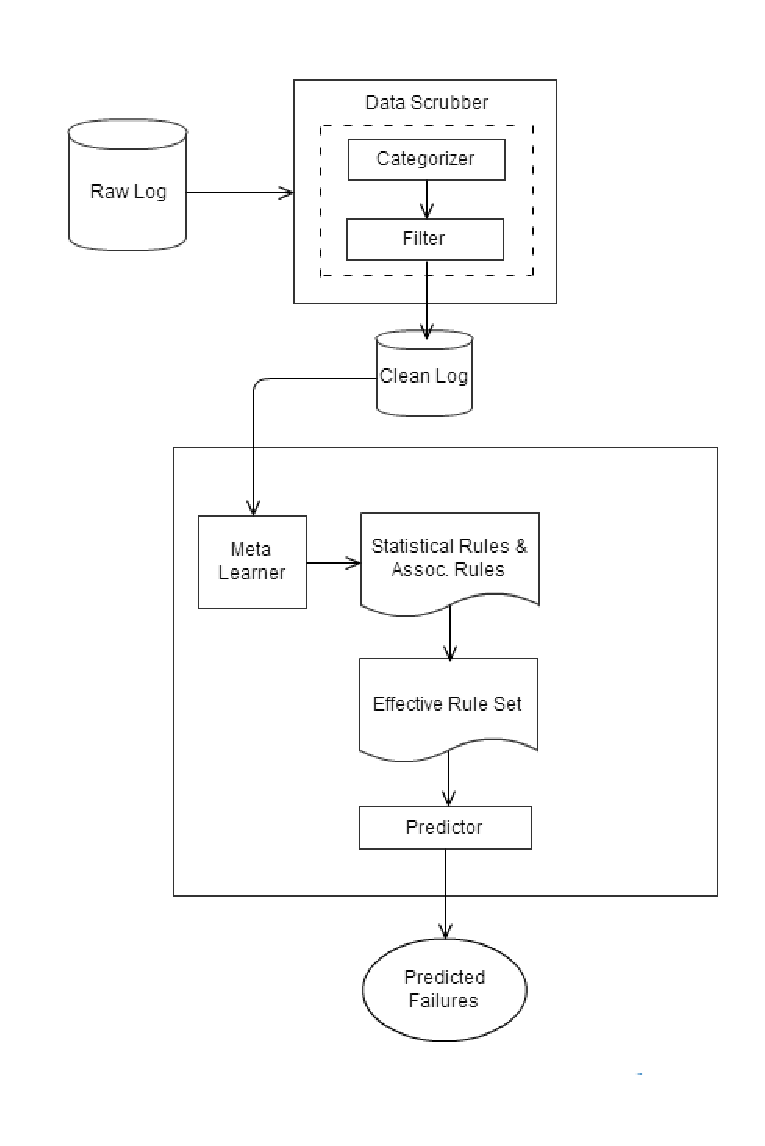
\includegraphics[width=10cm,height=10cm]{figures/failure_prediction_scheme.eps} 
			\caption{\small \sl Failure Prediction Scheme.\label{fig:Label7}} 
		\end{center} 
	\end{figure}

% Add cross reference.
\subsubsection{Data Scrubber}
The RAS logs cannot be used as is for data mining because of the unevenness in reporting the same type of error messages. The Data Scrubber handles all the actions of cleaning data so as to make it useable for mining. This steps also helps in reducing the amount of data storage spae required to store the statistical data. Upon completion, the data scrubber intends to provide a list of unique events for failure prediction. This operation is further divided into two parts:
\paragraph{Event Categorization}
The RAS log, has a lot of information and because of the inherant distributed nature of the Blue Gene/L System, the logs cannot be used as is. The logs originate from a variety of different facilities and carry a lot of information which needs to be made meaningful to the data mining program. We achieve this by categorizing events. Categorization of events maps the problem to a binary model where the particular event either occurs or not.

Event categorization is also done over the fatality of the event. This helps in recognizing failures efficiently.
\paragraph{Event Filtering}
The distributed nature of the system causes a lot of duplication in the logs.\cite{SCRUBBING_1}\cite{FAILURE_2} As the job is distributed across nodes, the same job reports the same type of events multiple times. By studying event duplication times, we decided upon a 300 sec threshold for temporal compression of data. Event logs that appeared from the same location within a 300 sec window having the same category field were reported only once.
\begin{figure}[t]
		\begin{center}
			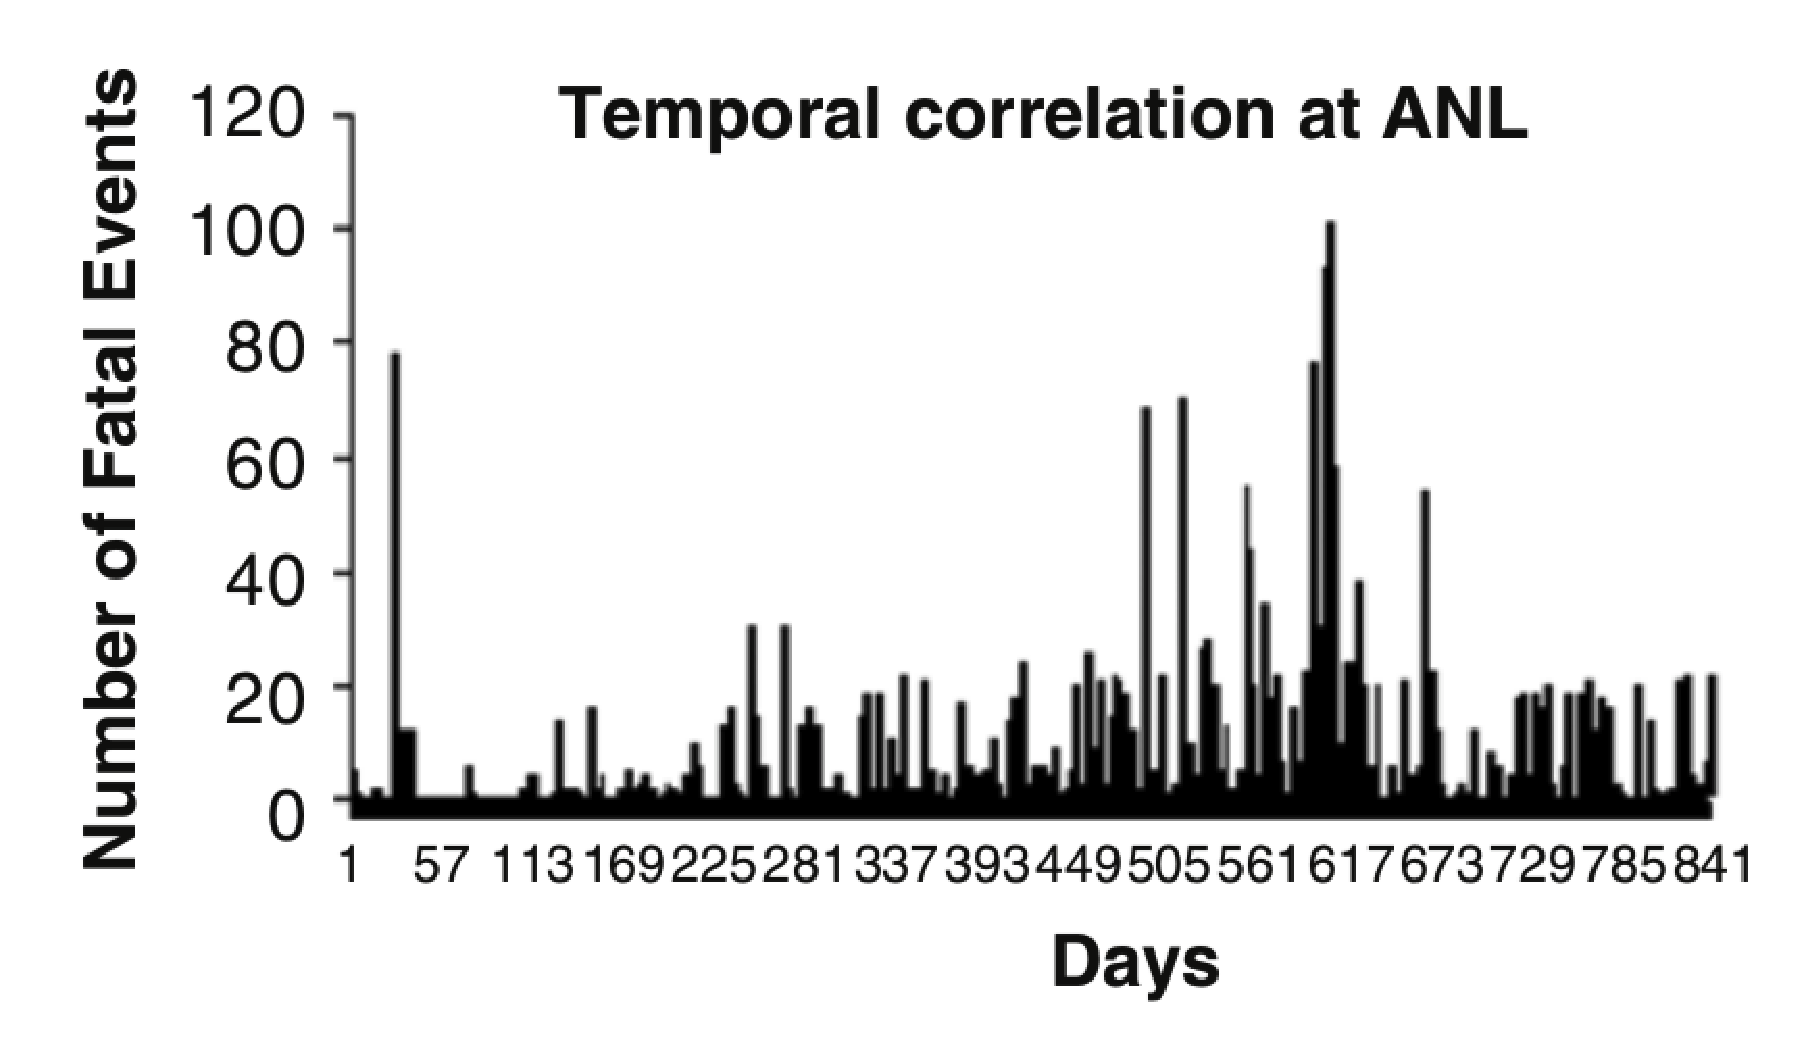
\includegraphics[width=10cm,height=7cm]{figures/temporal_correlation.eps} 
			\caption{\small \sl Temporal Correlation at ANL.\label{fig:Label7}} 
		\end{center} 
	\end{figure}


\subsection{Prediction}
The scrubbed data can now be processed by the the Prediction Scheme mechanism in the Fault Prediction Engine, to analyze the data logs for failure patterns and irregular entries. The techniques of Association Rule Based Learning are used for this prediction. The scrubbed data logs are fed to the Weka Data Mining Tool.\cite{WEKA} Weka is configured to find associations amongst the entries in the data log. The Apriori algorithm is preferred to other Association Rule Based Learning algorithms because it can be easily configured to work with the large datasets that we must work with.\cite{APRIORI_1}\cite{APRIORI_2} We set the parameters of "Apriori Associate" to a minimum support of 0.01 and a threshold confidence value of 0.1. Once Weka has finished the processing of the data logs, it returns a set of rules. These rules are supplied with confidence values and those with high confidence values for failure events are predicted to be possible future failures. Those events that can lead to failures with a high confidence value trigger the Automatic Healing Engine to migrate VMs and their processes from this compute node that is likely to fail to a compute node that is processing normally.
\begin{figure}[t]
		\begin{center}
			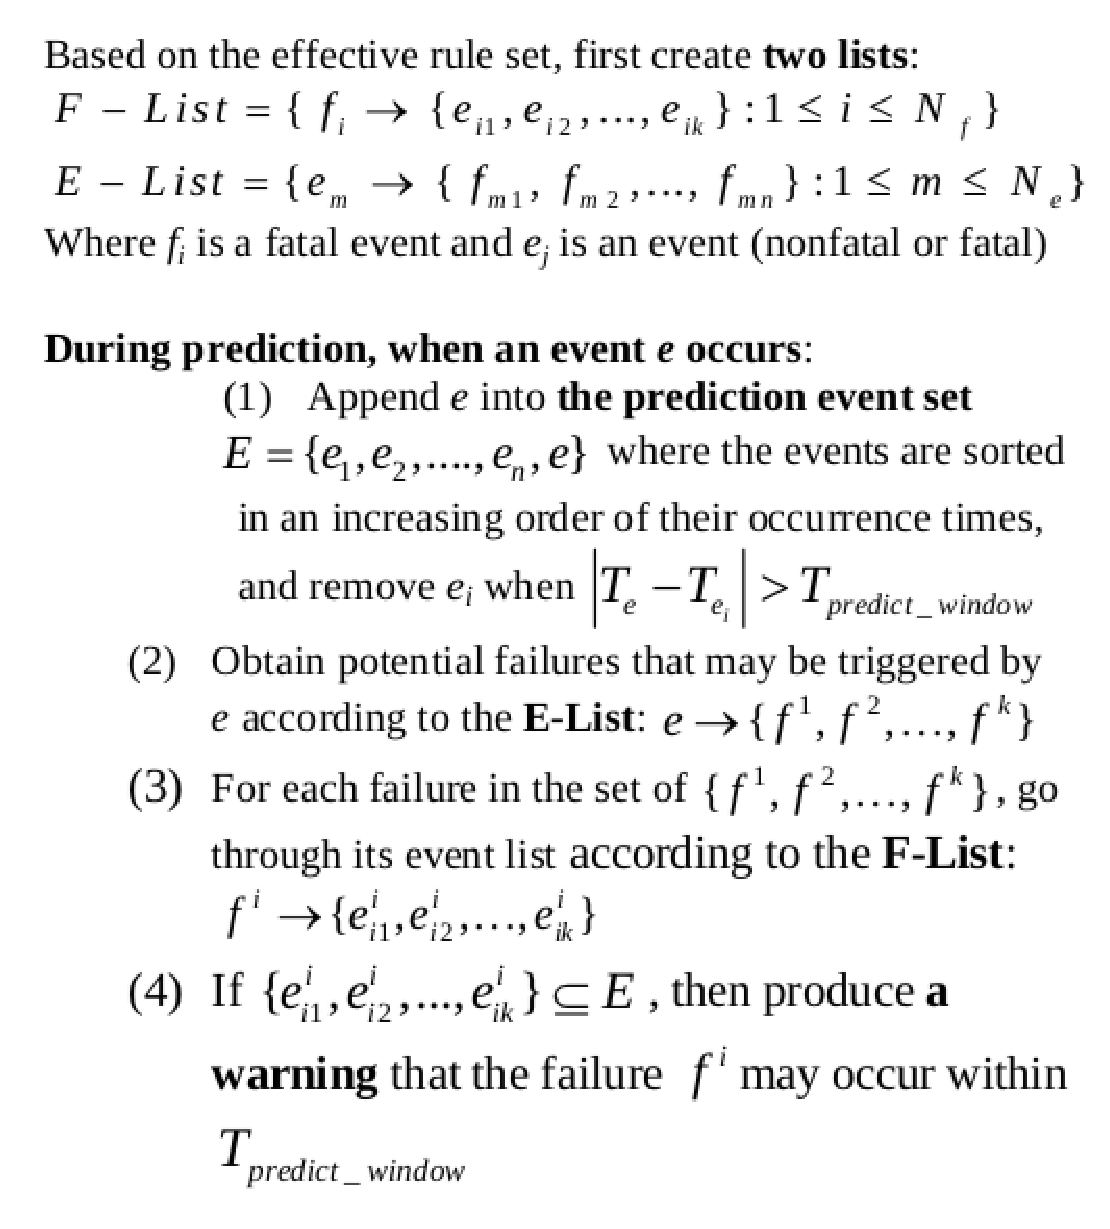
\includegraphics[width=8cm,height=10cm]{figures/prediction_algorithm.eps} 
			\caption{\small \sl Prediction Algorithm.\label{fig:Label8}} 
		\end{center} 
	\end{figure}
